\section{Tutoriais}

\subsection{Instalação}
\subsubsection{Linux}
Antes de iniciar a instalação, é uma boa prática verificar se o GCC já está instalado no seu sistema. Para fazer isso, abra um terminal e digite o seguinte comando:
\begin{minted}{bash}
  $ gcc --version
\end{minted}
Se o GCC já estiver instalado, você verá informações sobre a versão (Figura \ref{fig:versao_gcc}). Caso contrário, o terminal exibirá uma mensagem de erro.

\begin{figure}[H]
    \begin{center}
  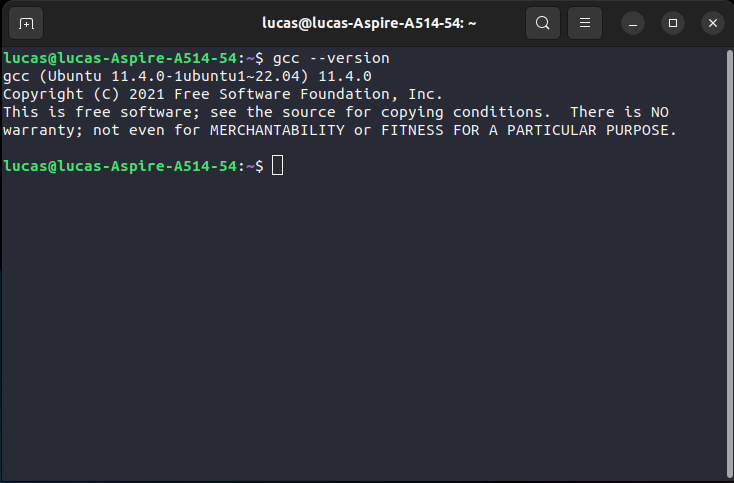
\includegraphics[width=450px]{imagens/versao_gcc.png}
  \end{center}
  \caption{Versão do GCC Sendo exibida no terminal}
  \label{fig:versao_gcc}
\end{figure}

Se o GCC não estiver instalado ou você desejar atualizá-lo para a versão mais recente, siga as etapas apropriadas para a sua distribuição Linux.

\paragraph{Ubuntu e Debian}
No Ubuntu e em sistemas baseados no Debian, você pode usar o \texttt{apt} para instalar o GCC. Abra um terminal e execute os seguintes comandos:
\begin{minted}{bash}
    $ sudo apt update
    $ sudo apt install build-essential
\end{minted}
O pacote \texttt{build-essential} inclui o GCC e outras ferramentas necessárias para compilar programas C.

\paragraph{CentOS e Fedora}
No CentOS e Fedora, você pode usar o \texttt{yum} ou \texttt{dnf} para instalar o GCC. Abra um terminal e execute os seguintes comandos:
\begin{minted}{bash}
    $ sudo yum groupinstall "Development Tools"
\end{minted}

\paragraph{Arch Linux}
No Arch Linux, você pode usar o \texttt{pacman} para instalar o GCC. Abra um terminal e execute o seguinte comando:

\begin{minted}{bash}
    $ sudo pacman -S gcc
\end{minted}

\subsubsection{Windows}
Agora, se você está usando o Windows, uma maneira conveniente de obter um compilador de C é através do Cygwin, que é uma coleção de ferramentas GNU e bibliotecas que fornecem funcionalidades semelhantes às encontradas em sistemas Linux.

Para instalar o Cygwin e o GCC (GNU Compiler Collection) no Windows, siga estas etapas:

\begin{enumerate}
\item Acesse o site oficial do Cygwin em \textbf{https://www.cygwin.com/}

\item Na página inicial do Cygwin, você encontrará um botão para baixar o instalador (normalmente chamado "setup-x86\_64.exe" para sistemas de 64 bits ou "setup-x86.exe" para sistemas de 32 bits). Baixe o instalador apropriado para o seu sistema.

\item Execute o instalador do Cygwin. O instalador irá guiá-lo pelo processo de instalação. Certifique-se de selecionar as opções relevantes, incluindo a seleção do local de instalação e os pacotes que deseja instalar. 

\item Quando chegar à tela de seleção de pacotes, pesquise "gcc" no campo de pesquisa e expanda a categoria "Devel" para encontrar o pacote "gcc-core". Marque a caixa de seleção ao lado dele.

\item Continue com o processo de instalação e o Cygwin instalará o GCC juntamente com outras ferramentas e bibliotecas necessárias.
\end{enumerate}

Para verificar se a instalação foi um sucesso, utilize no Prompt de Comando o seguinte comando que deverá retornar a versão do GCC:

\begin{minted}{bash}
    > gcc --version
\end{minted}

\subsection{Hello World}
Para começar, incluímos a biblioteca padrão de entrada e saída em C, chamada \texttt{<stdio.h>}, usando a diretiva de inclusão \texttt{\#include}.

Isso nos permite escrever o código dentro da função principal do arquivo. Na linguagem C, o código pode ser organizado em funções.

Uma função é um conjunto de comandos que executa uma tarefa específica em um módulo de código independente. A função é referenciada pelo programa principal através do nome atribuído a ela. O uso de funções é comum na programação estruturada, pois ajuda a modularizar o programa.

\begin{lstlisting}[language=C]
#include <stdio.h>

int main(){
    printf("Ola mundo.");
    return 0;
}
\end{lstlisting}

A função principal, denominada \texttt{main}, é uma função que retorna um valor inteiro e não aceita argumentos. O código do nosso programa é escrito dentro dessa função.

Dentro da função principal, usamos a função \texttt{printf}, que recebe uma string de formato como entrada, seguida por uma lista de valores, e produz uma string de saída que corresponde ao especificador de formato e aos valores de entrada fornecidos. Essa função permite exibir valores de qualquer tipo de dado na tela.

\begin{figure}[H]
    \begin{center}
  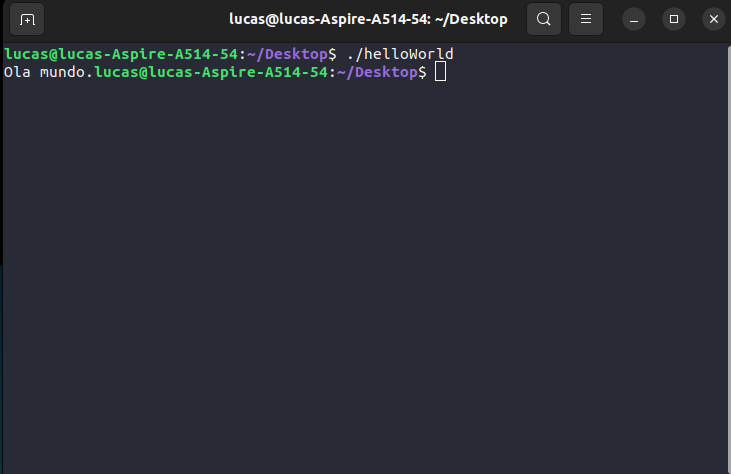
\includegraphics[width=450px]{imagens/hello_world.png}
  \end{center}
  \caption{"Hello World" executado}
  \label{fig:hello_world}
\end{figure}

É importante mencionar que a função principal deve retornar 0 para indicar que o programa foi executado com sucesso. Um retorno de 1 indica erro no código. Portanto, adicionamos a instrução \texttt{return 0;} no final da função principal.